\subsection{Solução}

Em resposta à necessidade dos LIMS aumentarem a eficiência de obtenção de dados, foi criada uma solução de workflows dinâmicos, que mudam a forma como as informações são apresentadas e disponibilizadas ao usuário.
Com uma interface adaptável e intuitiva, a solução permite ao usuários acessar e interagir com informações essenciais de maneira rápida e eficiente, melhorando a experiência do usuário.

O usuário tem a possibilidade de escolher, dentre todas as atividades disponíveis para sua visualização, a centralização da atividade escolhida para que ela seja o ponto central do fluxo de trabalho. Com isso, o usuário pode facilmente navegar para outras áreas relevantes da interface e personalizar o fluxo de trabalho de acordo com suas necessidades específicas de forma mais rápida do que seguindo o fluxo de trabalho original.

A rápida disponibilização de informações ao usuário resulta em uma série de ganhos, incluindo maior eficiência dos trabalhos feitos dentro do LIMS, já que workflows podem ser feitos com essa funcionalidade em mente, menor gasto com treinamento no uso do LIMS, já que uma interface dinâmica pode deixar a navegação mais intuitiva e aumento da produtividade do usuário com as informações disponibilizadas mais rapidamente.

O usuário deve, no entanto, saber onde as informações estão contidas dentro do fluxo do trabalho existente para selecionar a atividade correta que contém as informações desejadas. Com isso, a interface se altera para que o fluxo de trabalho seja centralizado na atividade que o usuário deseja.

As informações são disponibilizadas como se a atividade centralizada virasse a atividade inicial do workflow, ocorrendo um ``giro'' da atividade selecionada, transformando a atividades pais em atividades filhas da mesma, como podemos ver na figura~\ref{fig:primeira_implementacao}.

\begin{figure}
    \centering
    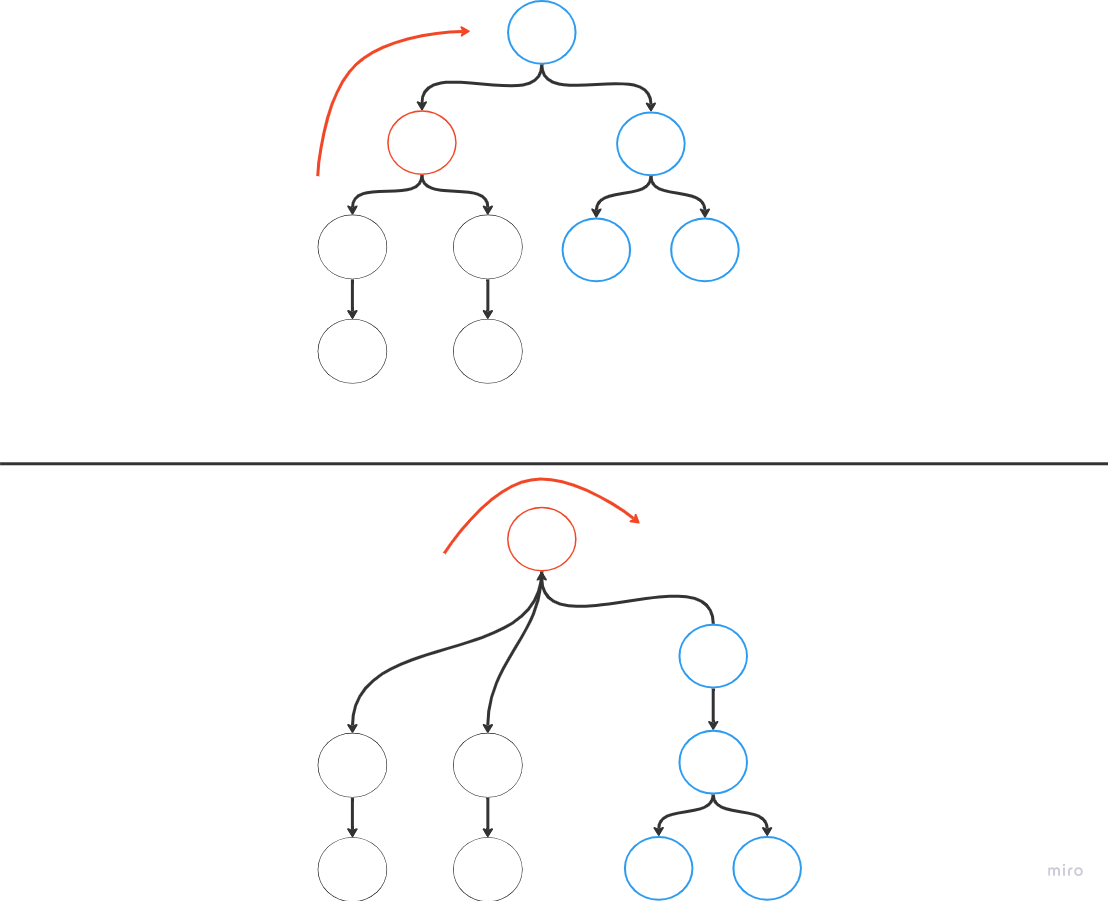
\includegraphics[width=1\textwidth]{imgs/Implementacoes/primeiraImplementacao.png}
    \caption{Representação da implementação de workflows dinâmicas. Na imagem de cima, podemos ver a implementação original de um workflow genérico que está prestes a ser reconstruído. A atividade em vermelho será utilizada como atividade focada apelo usuário. Com isso, a seta em vermelho representa o ``giro'' que o workflow faz para que a atividade selecionada vire a primeira atividade do workflow.}
    \label{fig:primeira_implementacao}
\end{figure}

\subsubsection{Mudanças no software para implementação de workflows dinâmicos}

Para que o Flux pudesse focar em uma atividade dentro do workflow, alteramos a definição de instância do programa. Anteriormente, instâncias eram definidas como o inicio do fluxo de trabalho do usuário para execução do BPM.

Com a implementação de workflows dinâmicos, foi necessário a utilização de instâncias como o ponto de partida de execução do usuário naquele momento, e não necessariamente o inicio do fluxo de trabalho. As instâncias agora demonstram, como ponto inicial, a atividade focada pelo usuário.

No software, instâncias ainda são criadas apenas para a atividade original, mantendo a ordenação do BPM, mas a disponibilização de informações é feita de maneira dinâmica, criando uma instância temporária onde a atividade inicial é a atividade selecionada pelo usuário, disponibilizando esta atividade centralizada como ponto de partida para sua execução.

Para selecionar qual atividade inicial será utilizada na visualização atual, foi alterada a interface para adicionar um seletor de atividades, disponibilizando todas as atividades que o usuário tem permissão de acessar em uma lista ordenada pelo nome da mesma. Nele, temos o nome de todas as atividades do workflow selecionado que o usuário tem a permissão de visualizar.

Caso o usuário não selecione nenhuma atividade, a atividade inicial utilizada será a padrão, deixando o workflow na visualização padrão. Exemplos para esta funcionalidade são mostrados na seção~\ref{sec:dinamic_workflows_examples}.

A árvore de atividades também teve de ser alterada, com a criação de novos tipos de atividades: Atividades pai, ou atividades anteriores. Neste tipo de atividade (Identificados pela cor azul na figura~\ref{fig:centrare_tree_normal_altered}), não é possível executar novas atividades, sendo existentes apenas por motivos de disponibilização de informações pertinentes à execução atual.

Foi necessário a criação deste novo tipo de atividade para disponibilizar informações de atividades anteriores para o usuário, já que as informações podem ser pertinentes para o usuário.

Na mesma figura~\ref{fig:centrare_tree_normal_altered} temos as informações do paciente como primeira atividade da visualização original, podendo ser necessária para preenchimento de próximas atividades da atividade selecionada ``Cirurgia de Nariz''.

\begin{figure}
    \centering
    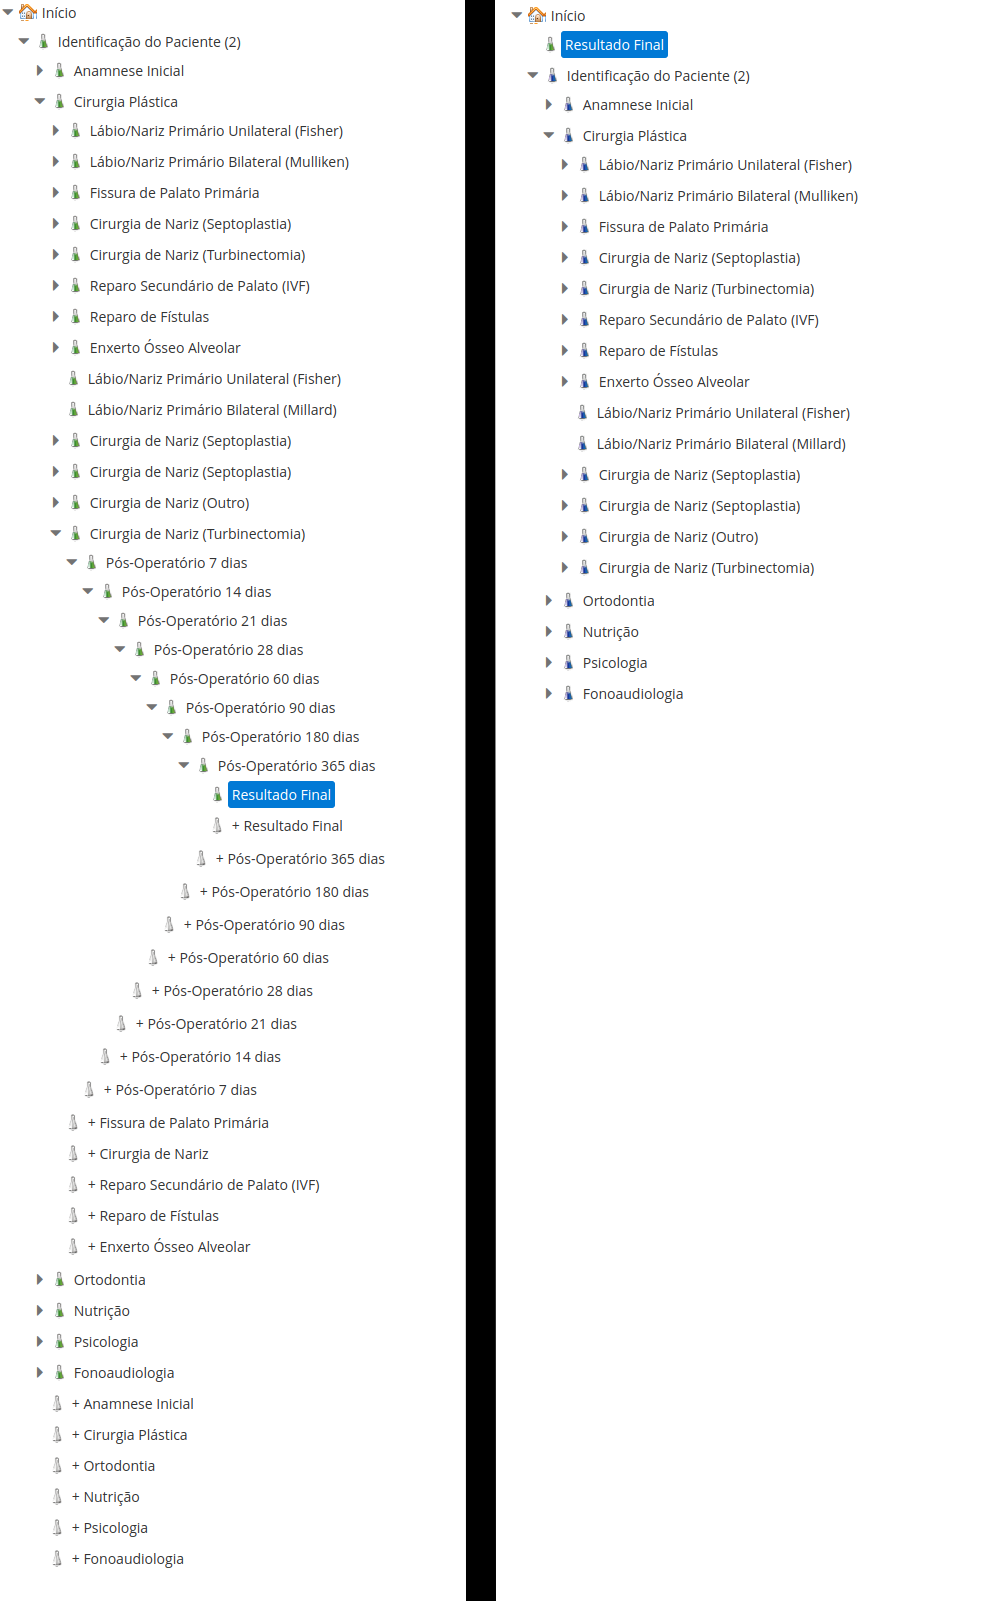
\includegraphics[height=1\textwidth]{imgs/CENTRARE/arvoreNormalEAlterada.png}
    \caption{Imagem demonstrando a árvore de atividades no software original (Esquerda) e a árvore de atividades alterada (Direita). Como podemos ver, a atividade selecionada na esquerda que está no meio do workflow é a mesma atividade selecionada na direita, que agora virou a atividade focada por seleção do usuário. Atividades pai são demonstradas em azul, disponibilizando todas as informações existentes mesmo com a alteração do foco do workflow.}
    \label{fig:centrare_tree_normal_altered}
\end{figure}